\documentclass{article}
\usepackage[T1]{fontenc}
\usepackage[portrait]{geometry}
\geometry{verbose,tmargin=1cm,bmargin=1cm,lmargin=3cm,rmargin=3cm}
\setlength{\parskip}{0in}
\setlength{\parindent}{0pt}
\usepackage{url}
\usepackage[unicode=true,pdfusetitle,
 bookmarks=true,bookmarksnumbered=false,bookmarksopen=false,
 breaklinks=false,pdfborder={3 1 1},backref=false,colorlinks=false]
 {hyperref}



\usepackage{Sweave}
\begin{document}

\Sconcordance{concordance:probabilities.tex:probabilities.Rnw:%
1 14 1 1 0 47 1 1 16 3 0 1 1 2 0 1 10 2 0 1 1 2 0 1 1 2 0 1 8 2 0 1 1 2 %
0 1 1 2 0 1 8 10 0 1 3 3 1 1 8 1 3 2 1 1 16 3 0 1 1 2 0 1 7 2 0 1 1 2 0 %
1 6 2 0 1 1 2 0 1 1 2 0 1 6 10 0 1 3 2 1 1 8 1 3 3 1}


\title{Probabilities of significance}

\author{Mc}
\maketitle
\section*{Reference}
Based on Meetings note
 
(\href{https://docs.google.com/document/d/1zhUdzu9HjuZ8tqvLVKh6QoqIphHgWVrIHosbvRAGGvs/edit}{ "Meetings for Significance \& Accuracy"}, 24-02-06 

\section*{What's new}

We plot the probabilities of an indicator to be significant as follows:
\begin{itemize}
\item [{1}] 
\begin{itemize}
\item [{a.}] Either continuous or categorical are significant 
\item [{b.}] Continuous significant (ignoring categorical) 
\item [{c.}] Categorical significant (ignoring continuous) 
\end{itemize}
\item [{2}] 
\begin{itemize}
\item [{a.}] Only continuous significant 
\item [{b.}] Only categorical significant 
\item [{c.}] Both continuous and categorical are significant 
\item [{d.}] Neither continuous and categorical are significant 
 
\end{itemize}
 
\end{itemize}

\section*{Introduction}
In simulations we checked the propability of an indicator (continuous or media-split) as the probability (frequency of runs) of being significant when it should be (latent effect size is greater than zero) over the probability of being significant when it should be not.
\section*{Setup}
\subsection*{Model}
Two continuous latent variables (\(\eta\) and \(\xi\) ) are created with N cases, sharing a correlation equal to \(\rho\). A measure \(x\) of \(\xi\) is created with reliability \(rel\), and then  is dichotomized accordingly to \(p\) \(1-p\) into \(c\). The correlations \( r_pe=r(\eta,x) \)  and \( r_pb=r(\eta,c) \) are computed, their p-value and significance (at .05) is recorded.
\subsection*{Design}
\(\rho=(0,.1,.2,.3,.4,.5,.6,.7) \)
\(rel=(0.3, 0.4 ,0.5, 0.6, 0.7 ,0.8 0.9) \) 

\subsection*{Propabilities as a functions of \(\rho\)}

The computation follows Jamie's computation at the last meeting. The probabilities are the following: \(f_0\) is the number of times the indicator was significant when the null hypothesis was true, \(f_1\) is the probability of being the only one significant for a given \(\rho)>0\). The probability \(P\) is \(P= f_1 \over (f_1+f_0 \))  


\begin{Schunk}
\begin{Soutput}
Number of times Either Continuos or Categorical was significant under the null hypothesis
\end{Soutput}
\begin{Soutput}
[1] 562
\end{Soutput}
\begin{Soutput}
Number of times Continuous was significant under the null hypothesis
\end{Soutput}
\begin{Soutput}
[1] 345
\end{Soutput}
\begin{Soutput}
P of  Continuos  significant under true hypotheses
\end{Soutput}
\begin{Soutput}
Number of times Categorical was significant under the null hypothesis
\end{Soutput}
\begin{Soutput}
[1] 351
\end{Soutput}
\begin{Soutput}
P of  categorical  significant under true hypotheses
\end{Soutput}
\begin{Soutput}
  rho continuous categorical    either
1 0.1  0.6805556   0.6265957 0.6341146
2 0.2  0.8359486   0.7817164 0.7844265
3 0.3  0.9015130   0.8707658 0.8585096
4 0.4  0.9251302   0.9038356 0.8874199
5 0.5  0.9359688   0.9241081 0.9025490
6 0.6  0.9417918   0.9332573 0.9104525
7 0.7  0.9459078   0.9395245 0.9161069
\end{Soutput}
\end{Schunk}


\subsubsection*{Figure 1: Probability of being significance}

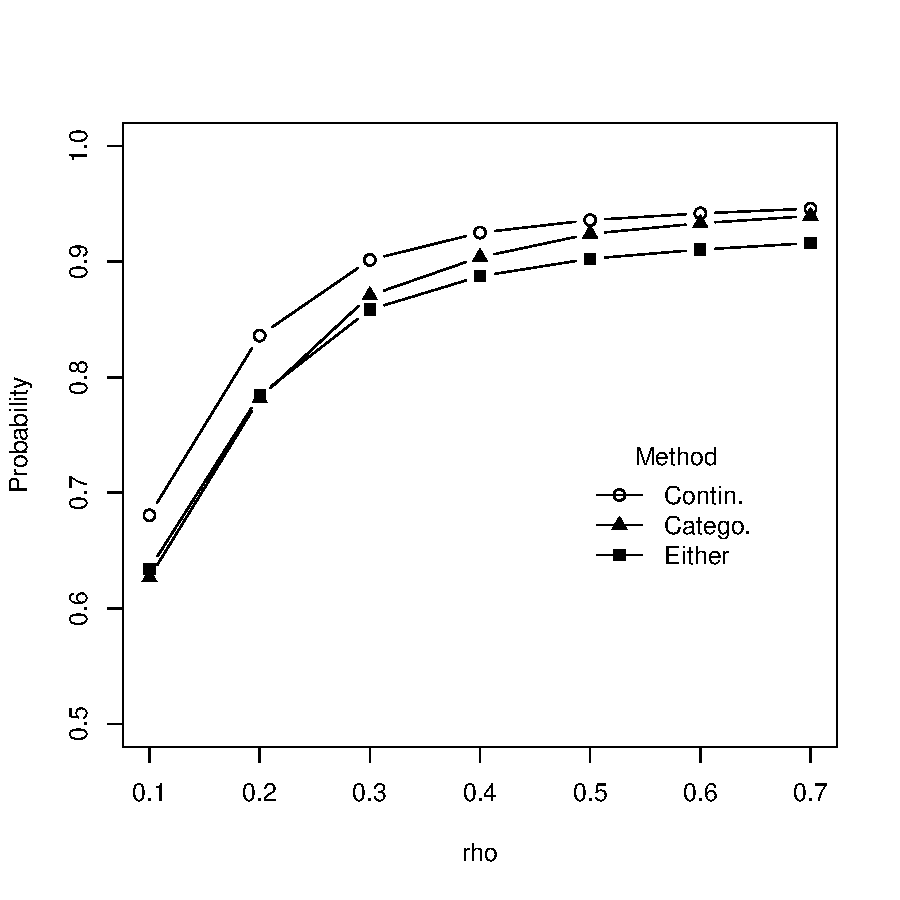
\includegraphics{probabilities-t2}



\begin{Schunk}
\begin{Soutput}
Number of times both Continuos and Categorical were significant under the null hypothesis
\end{Soutput}
\begin{Soutput}
[1] 134
\end{Soutput}
\begin{Soutput}
Number of times only Continuos was significant under the null hypothesis
\end{Soutput}
\begin{Soutput}
[1] 211
\end{Soutput}
\begin{Soutput}
Number of times only Categorical was significant under the null hypothesis
\end{Soutput}
\begin{Soutput}
[1] 217
\end{Soutput}
\begin{Soutput}
Odds of only Continuos  significant under true hypotheses
\end{Soutput}
\begin{Soutput}
  rho continuous categorical      both
1 0.1  0.6459732   0.5241228 0.7231405
2 0.2  0.7887888   0.5694444 0.8786232
3 0.3  0.8320064   0.5373134 0.9403649
4 0.4  0.8427720   0.4348958 0.9589712
5 0.5  0.8152364   0.4274406 0.9684409
6 0.6  0.7925270   0.3782235 0.9727088
7 0.7  0.7642458   0.3239875 0.9755608
\end{Soutput}
\end{Schunk}

\subsubsection*{Figure 2: Probs. of being significant}

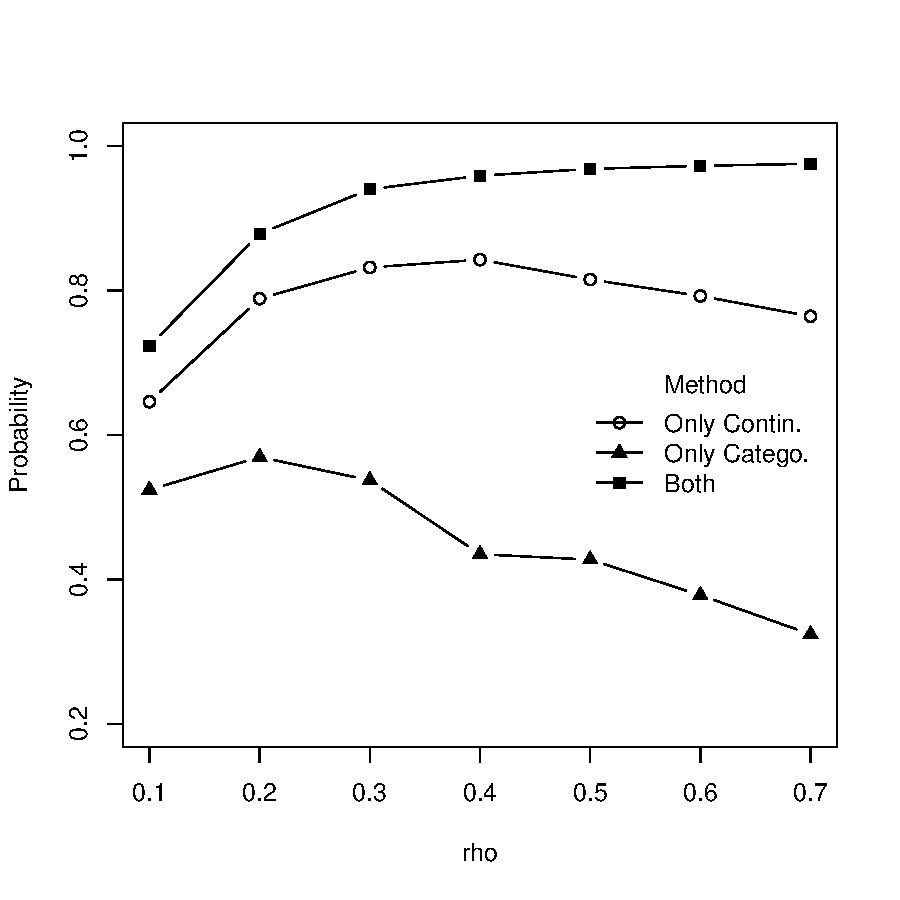
\includegraphics{probabilities-t4}



\end{document}
